\batchmode
\documentclass{book}
\usepackage[a4paper,top=2.5cm,bottom=2.5cm,left=2.5cm,right=2.5cm]{geometry}
\usepackage{makeidx}
\usepackage{natbib}
\usepackage{graphicx}
\usepackage{multicol}
\usepackage{float}
\usepackage{listings}
\usepackage{color}
\usepackage{ifthen}
\usepackage[table]{xcolor}
\usepackage{textcomp}
\usepackage{alltt}
\usepackage[utf8]{inputenc}
\usepackage{mathptmx}
\usepackage[scaled=.90]{helvet}
\usepackage{courier}
\usepackage{sectsty}
\usepackage{amssymb}
\usepackage[titles]{tocloft}
\usepackage{doxygen}
\lstset{language=C++,inputencoding=utf8,basicstyle=\footnotesize,breaklines=true,breakatwhitespace=true,tabsize=8,numbers=left }
\makeindex
\setcounter{tocdepth}{3}
\renewcommand{\footrulewidth}{0.4pt}
\renewcommand{\familydefault}{\sfdefault}
\hfuzz=15pt
\setlength{\emergencystretch}{15pt}
\hbadness=750
\tolerance=750
\begin{document}
\begin{titlepage}
\vspace*{7cm}
\begin{center}
{\Large Grijper }\\
\vspace*{1cm}
{\large Generated by Doxygen 1.8.3.1}\\
\vspace*{0.5cm}
{\small Tue Sep 24 2013 15:54:29}\\
\end{center}
\end{titlepage}
\clearemptydoublepage
\pagenumbering{roman}
\tableofcontents
\clearemptydoublepage
\pagenumbering{arabic}
\chapter{Main Page}
\label{index}

{\bfseries Grijper} 

--$>$ 
\chapter{File Index}
\section{File List}
Here is a list of all files with brief descriptions\-:\begin{DoxyCompactList}
\item\contentsline{section}{{\bf command.\-h} }{\pageref{command_8h}}{}
\item\contentsline{section}{{\bf console.\-cpp} }{\pageref{console_8cpp}}{}
\item\contentsline{section}{{\bf gripper\-\_\-actuator.\-cpp} }{\pageref{gripper__actuator_8cpp}}{}
\item\contentsline{section}{{\bf gripper\-\_\-controller.\-cpp} }{\pageref{gripper__controller_8cpp}}{}
\item\contentsline{section}{{\bf phidget\-\_\-reader.\-cpp} }{\pageref{phidget__reader_8cpp}}{}
\item\contentsline{section}{{\bf rviz\-\_\-gripper.\-cpp} }{\pageref{rviz__gripper_8cpp}}{}
\item\contentsline{section}{{\bf rviz\-\_\-object.\-cpp} }{\pageref{rviz__object_8cpp}}{}
\end{DoxyCompactList}

\chapter{File Documentation}
\section{gripper\-\_\-actuator.\-cpp File Reference}
\label{gripper__actuator_8cpp}\index{gripper\-\_\-actuator.\-cpp@{gripper\-\_\-actuator.\-cpp}}
{\ttfamily \#include $<$ros/ros.\-h$>$}\\*
{\ttfamily \#include $<$std\-\_\-msgs/\-Float32.\-h$>$}\\*
{\ttfamily \#include $<$sstream$>$}\\*
{\ttfamily \#include $<$stdio.\-h$>$}\\*
{\ttfamily \#include $<$threemxl/\-C3mxl\-R\-O\-S.\-h$>$}\\*
{\ttfamily \#include $<$threemxl/\-C\-Dynamixel\-R\-O\-S.\-h$>$}\\*
Include dependency graph for gripper\-\_\-actuator.\-cpp\-:
\nopagebreak
\begin{figure}[H]
\begin{center}
\leavevmode
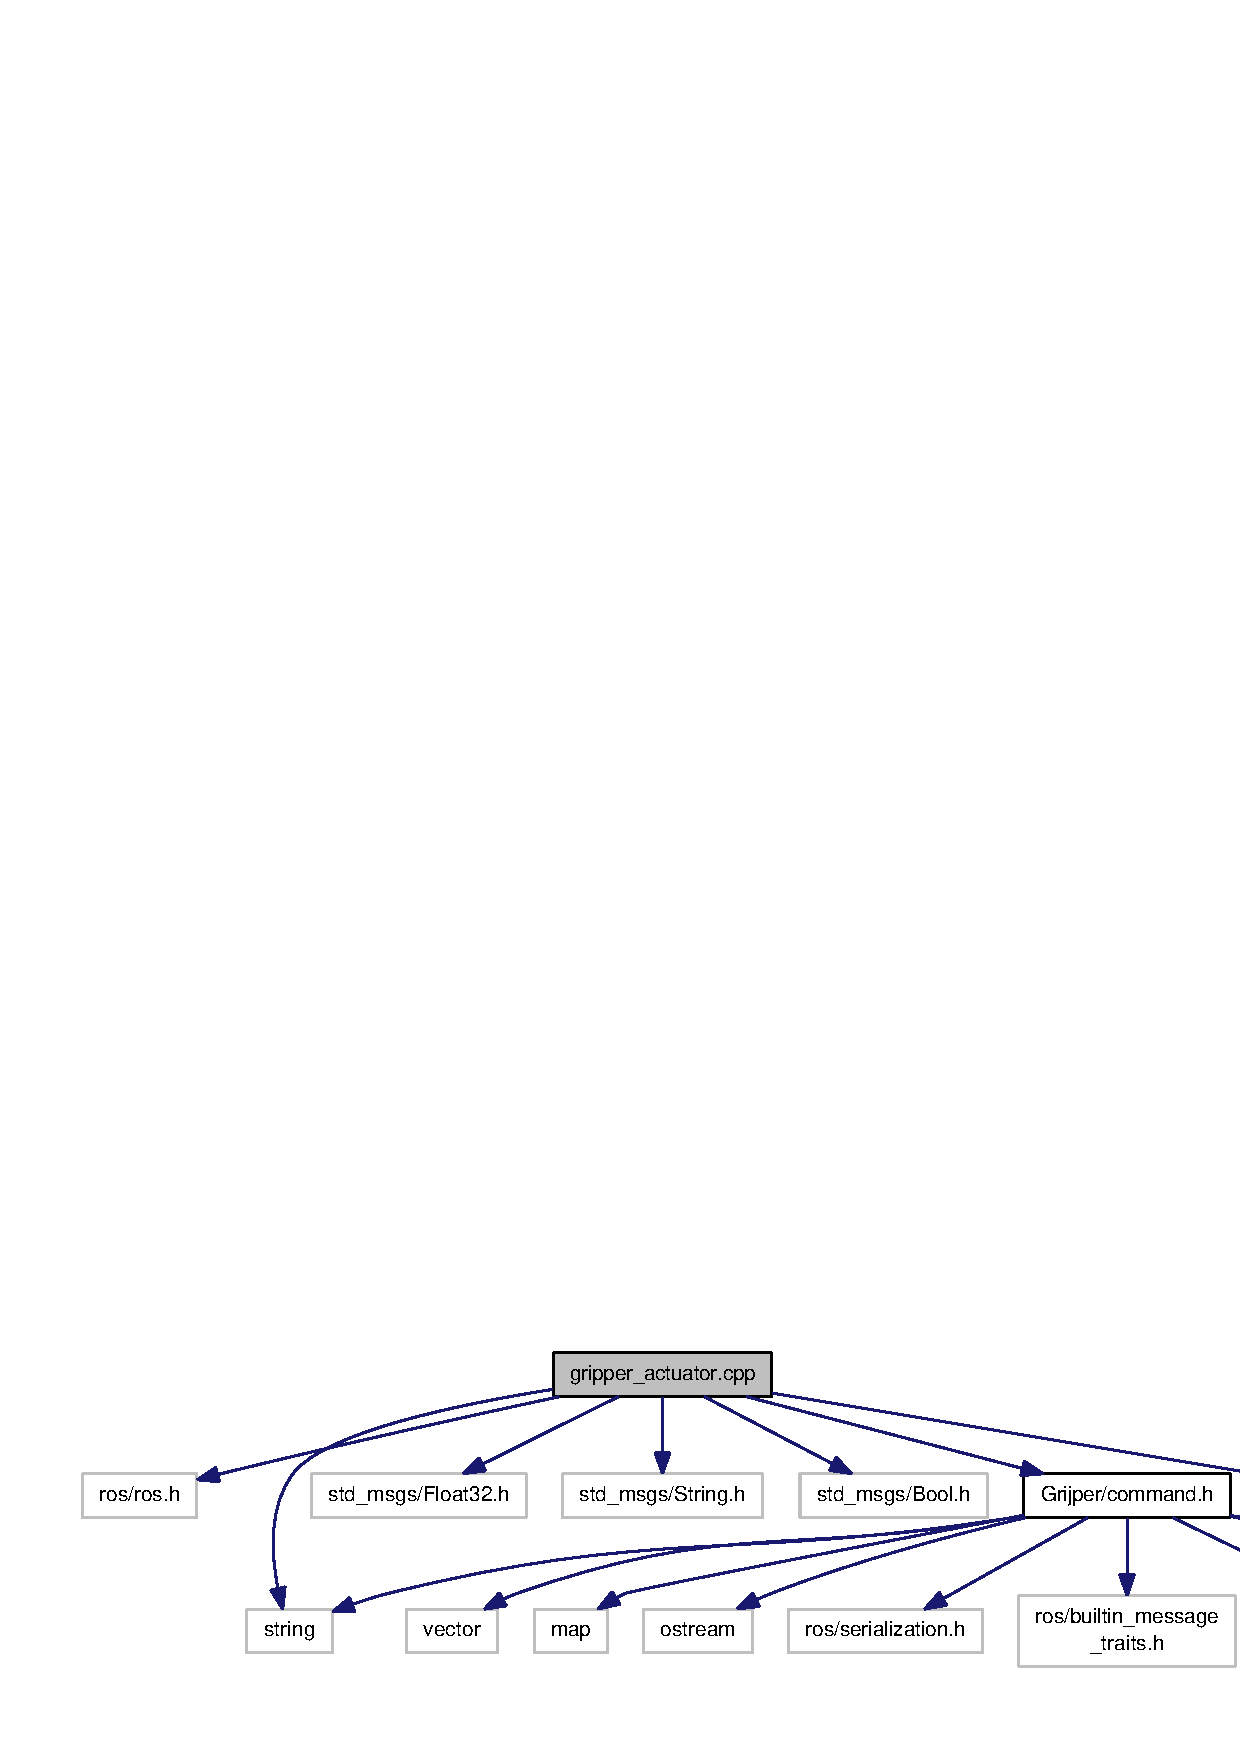
\includegraphics[width=350pt]{gripper__actuator_8cpp__incl}
\end{center}
\end{figure}
\subsection*{Macros}
\begin{DoxyCompactItemize}
\item 
\#define {\bf D\-X\-L\-C\-\_\-\-S\-A\-F\-E\-\_\-\-C\-A\-L\-L}(call)
\end{DoxyCompactItemize}
\subsection*{Functions}
\begin{DoxyCompactItemize}
\item 
bool {\bf close} (float)
\item 
bool {\bf execute} (Arg\-List)
\item 
void {\bf gripper\-Actuate} (const std\-\_\-msgs\-::\-Float32\-::\-Const\-Ptr \&)
\item 
void {\bf gripper\-Control} (const std\-\_\-msgs\-::\-String\-::\-Const\-Ptr \&)
\item 
int {\bf main} (int argc, char $\ast$$\ast$argv)
\item 
bool {\bf open} ()
\end{DoxyCompactItemize}
\subsection*{Variables}
\begin{DoxyCompactItemize}
\item 
ros\-::\-Publisher {\bf publisher}
\end{DoxyCompactItemize}


\subsection{Macro Definition Documentation}
\index{gripper\-\_\-actuator.\-cpp@{gripper\-\_\-actuator.\-cpp}!D\-X\-L\-C\-\_\-\-S\-A\-F\-E\-\_\-\-C\-A\-L\-L@{D\-X\-L\-C\-\_\-\-S\-A\-F\-E\-\_\-\-C\-A\-L\-L}}
\index{D\-X\-L\-C\-\_\-\-S\-A\-F\-E\-\_\-\-C\-A\-L\-L@{D\-X\-L\-C\-\_\-\-S\-A\-F\-E\-\_\-\-C\-A\-L\-L}!gripper_actuator.cpp@{gripper\-\_\-actuator.\-cpp}}
\subsubsection[{D\-X\-L\-C\-\_\-\-S\-A\-F\-E\-\_\-\-C\-A\-L\-L}]{\setlength{\rightskip}{0pt plus 5cm}\#define D\-X\-L\-C\-\_\-\-S\-A\-F\-E\-\_\-\-C\-A\-L\-L(
\begin{DoxyParamCaption}
\item[{}]{call}
\end{DoxyParamCaption}
)}\label{gripper__actuator_8cpp_a3cdecab00d916e74baf9ca4b8a8fd4f1}
{\bfseries Value\-:}
\begin{DoxyCode}
\textcolor{keywordflow}{do} \{ \(\backslash\)
    int ret = call; \(\backslash\)
    if (ret != DXL\_SUCCESS) \{ \(\backslash\)
      cout << \textcolor{stringliteral}{"Error:"} << endl << \textcolor{stringliteral}{"  "} << C3mxl::translateErrorCode(ret) << \textcolor{stringliteral}{" (0x"} << hex << ret << dec << \textcolor{stringliteral}{
      ")"} << endl; \(\backslash\)
    \} \(\backslash\)
  \} \textcolor{keywordflow}{while} (0)
\end{DoxyCode}


Definition at line 20 of file gripper\-\_\-actuator.\-cpp.



\subsection{Function Documentation}
\index{gripper\-\_\-actuator.\-cpp@{gripper\-\_\-actuator.\-cpp}!close@{close}}
\index{close@{close}!gripper_actuator.cpp@{gripper\-\_\-actuator.\-cpp}}
\subsubsection[{close}]{\setlength{\rightskip}{0pt plus 5cm}bool close (
\begin{DoxyParamCaption}
\item[{float}]{force}
\end{DoxyParamCaption}
)}\label{gripper__actuator_8cpp_a60598c74e06026d9314d3362a1629936}


Definition at line 58 of file gripper\-\_\-actuator.\-cpp.

\index{gripper\-\_\-actuator.\-cpp@{gripper\-\_\-actuator.\-cpp}!execute@{execute}}
\index{execute@{execute}!gripper_actuator.cpp@{gripper\-\_\-actuator.\-cpp}}
\subsubsection[{execute}]{\setlength{\rightskip}{0pt plus 5cm}bool execute (
\begin{DoxyParamCaption}
\item[{Arg\-List}]{args}
\end{DoxyParamCaption}
)}\label{gripper__actuator_8cpp_a8002ba95eddc1ad1aeb79d6ac8142156}


Definition at line 50 of file gripper\-\_\-actuator.\-cpp.

\index{gripper\-\_\-actuator.\-cpp@{gripper\-\_\-actuator.\-cpp}!gripper\-Actuate@{gripper\-Actuate}}
\index{gripper\-Actuate@{gripper\-Actuate}!gripper_actuator.cpp@{gripper\-\_\-actuator.\-cpp}}
\subsubsection[{gripper\-Actuate}]{\setlength{\rightskip}{0pt plus 5cm}void gripper\-Actuate (
\begin{DoxyParamCaption}
\item[{const std\-\_\-msgs\-::\-Float32\-::\-Const\-Ptr \&}]{msg}
\end{DoxyParamCaption}
)}\label{gripper__actuator_8cpp_a45524816df9f7663ba360599b42a36af}


Definition at line 40 of file gripper\-\_\-actuator.\-cpp.

\index{gripper\-\_\-actuator.\-cpp@{gripper\-\_\-actuator.\-cpp}!gripper\-Control@{gripper\-Control}}
\index{gripper\-Control@{gripper\-Control}!gripper_actuator.cpp@{gripper\-\_\-actuator.\-cpp}}
\subsubsection[{gripper\-Control}]{\setlength{\rightskip}{0pt plus 5cm}void gripper\-Control (
\begin{DoxyParamCaption}
\item[{const std\-\_\-msgs\-::\-String\-::\-Const\-Ptr \&}]{msg}
\end{DoxyParamCaption}
)}\label{gripper__actuator_8cpp_a101b2140b24b7e4ae8ffa902e5e8b371}


Definition at line 45 of file gripper\-\_\-actuator.\-cpp.

\index{gripper\-\_\-actuator.\-cpp@{gripper\-\_\-actuator.\-cpp}!main@{main}}
\index{main@{main}!gripper_actuator.cpp@{gripper\-\_\-actuator.\-cpp}}
\subsubsection[{main}]{\setlength{\rightskip}{0pt plus 5cm}int main (
\begin{DoxyParamCaption}
\item[{int}]{argc, }
\item[{char $\ast$$\ast$}]{argv}
\end{DoxyParamCaption}
)}\label{gripper__actuator_8cpp_a3c04138a5bfe5d72780bb7e82a18e627}


Definition at line 28 of file gripper\-\_\-actuator.\-cpp.

\index{gripper\-\_\-actuator.\-cpp@{gripper\-\_\-actuator.\-cpp}!open@{open}}
\index{open@{open}!gripper_actuator.cpp@{gripper\-\_\-actuator.\-cpp}}
\subsubsection[{open}]{\setlength{\rightskip}{0pt plus 5cm}bool open (
\begin{DoxyParamCaption}
{}
\end{DoxyParamCaption}
)}\label{gripper__actuator_8cpp_adb20eae91802d6ad6366cdee0220c280}


Definition at line 54 of file gripper\-\_\-actuator.\-cpp.



\subsection{Variable Documentation}
\index{gripper\-\_\-actuator.\-cpp@{gripper\-\_\-actuator.\-cpp}!publisher@{publisher}}
\index{publisher@{publisher}!gripper_actuator.cpp@{gripper\-\_\-actuator.\-cpp}}
\subsubsection[{publisher}]{\setlength{\rightskip}{0pt plus 5cm}ros\-::\-Publisher publisher}\label{gripper__actuator_8cpp_adde9f51ddf0fb5c82c57b4075b6e9400}


Definition at line 15 of file gripper\-\_\-actuator.\-cpp.


\section{gripper\-\_\-controller.\-cpp File Reference}
\label{gripper__controller_8cpp}\index{gripper\-\_\-controller.\-cpp@{gripper\-\_\-controller.\-cpp}}
{\ttfamily \#include $<$ros/ros.\-h$>$}\\*
{\ttfamily \#include $<$cmath$>$}\\*
{\ttfamily \#include $<$string$>$}\\*
{\ttfamily \#include $<$std\-\_\-msgs/\-Float32.\-h$>$}\\*
{\ttfamily \#include $<$std\-\_\-msgs/\-Bool.\-h$>$}\\*
{\ttfamily \#include $<$std\-\_\-msgs/\-String.\-h$>$}\\*
{\ttfamily \#include $<$Grijper/command.\-h$>$}\\*
Include dependency graph for gripper\-\_\-controller.\-cpp\-:\nopagebreak
\begin{figure}[H]
\begin{center}
\leavevmode
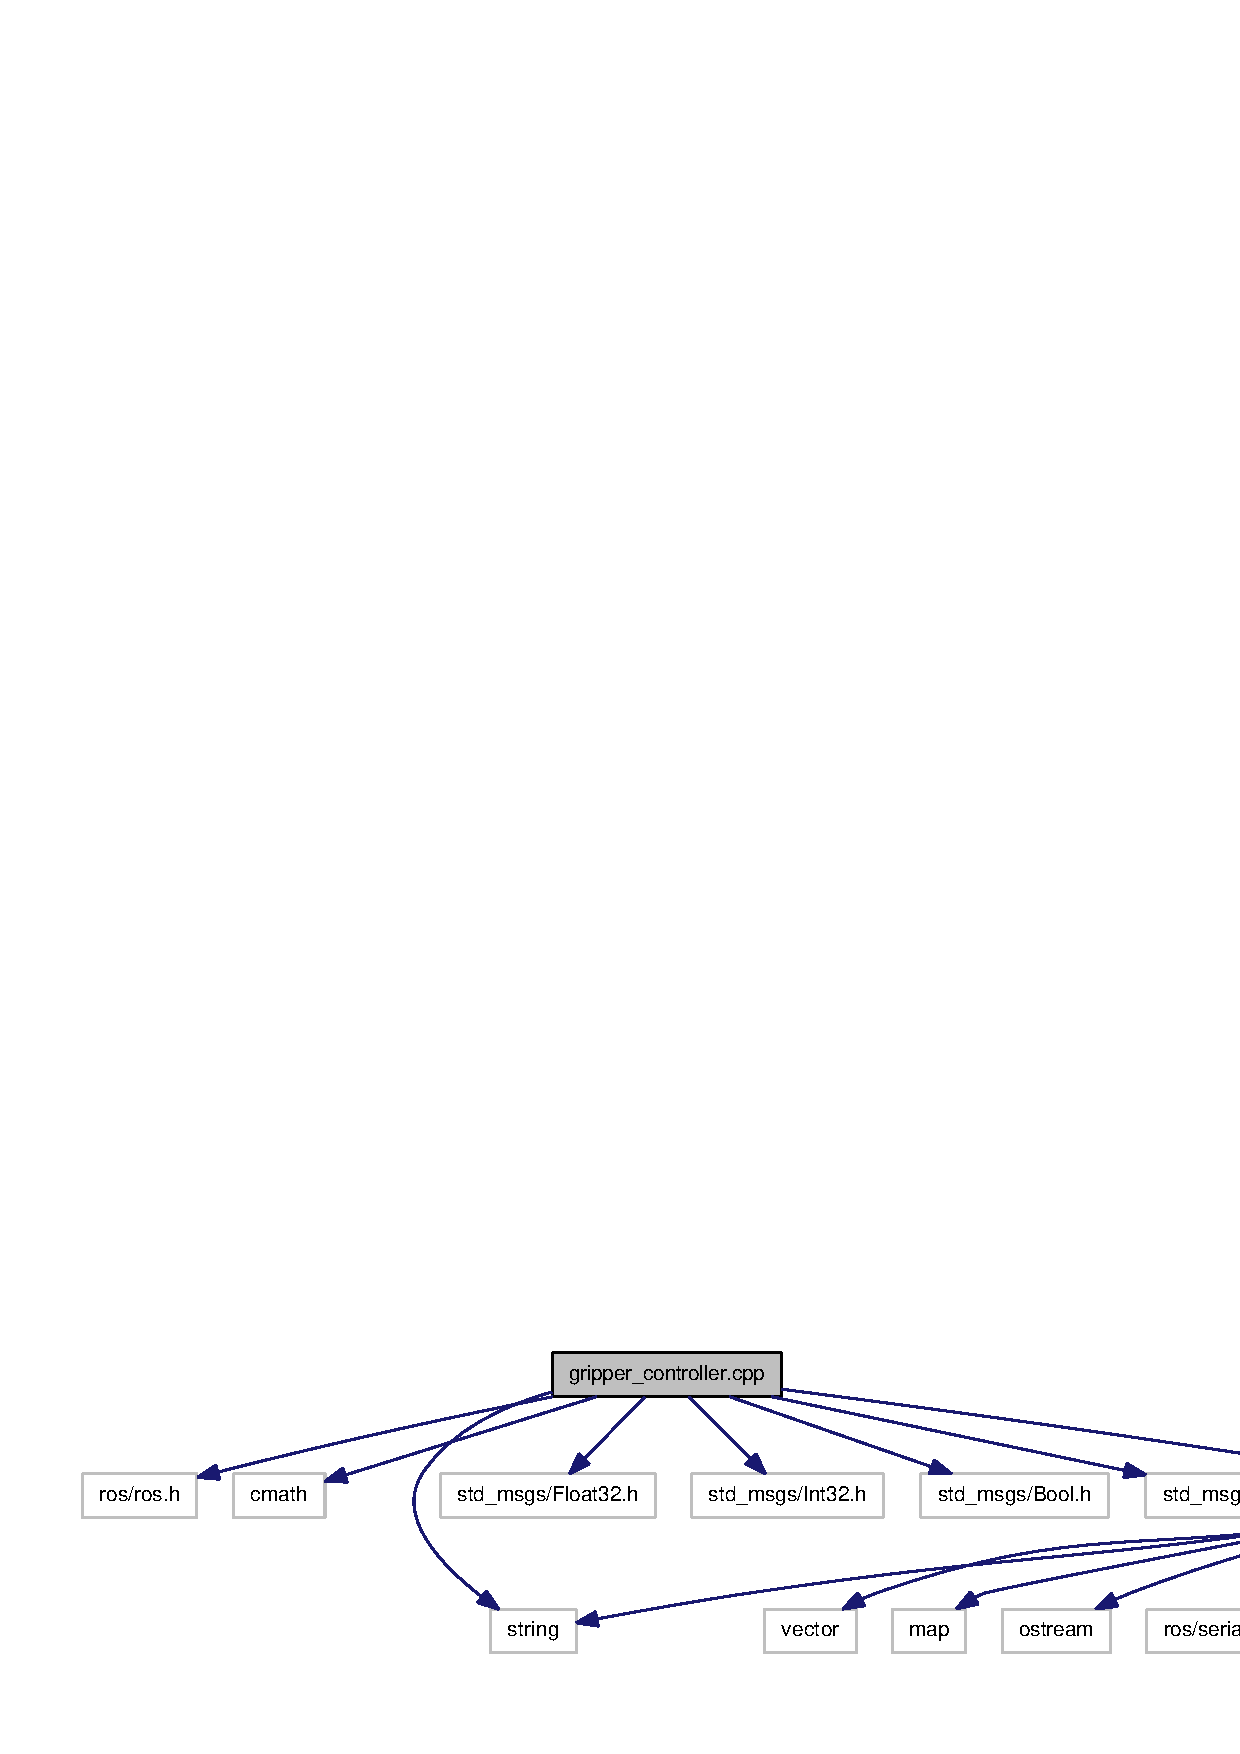
\includegraphics[width=350pt]{gripper__controller_8cpp__incl}
\end{center}
\end{figure}
\subsection*{Functions}
\begin{DoxyCompactItemize}
\item 
bool {\bf close\-\_\-gripper} (float distance)
\begin{DoxyCompactList}\small\item\em Small evaluation method to see if the gripper should be closed. \end{DoxyCompactList}\item 
void {\bf gripper\-Command} (const std\-\_\-msgs\-::\-String\-::\-Const\-Ptr \&msg)
\begin{DoxyCompactList}\small\item\em Method for evaluating and executing commands received from the console. \end{DoxyCompactList}\item 
void {\bf gripper\-Phidget} (const std\-\_\-msgs\-::\-Float32\-::\-Const\-Ptr \&msg)
\begin{DoxyCompactList}\small\item\em Method that evaluates the phidget sensor values and takes appropriate action. \end{DoxyCompactList}\item 
int {\bf main} (int argc, char $\ast$$\ast$argv)
\begin{DoxyCompactList}\small\item\em Main method of the controller node. All incoming messages are analysed and commands are sent from this node. \end{DoxyCompactList}\item 
bool {\bf open\-\_\-gripper} (float distance)
\begin{DoxyCompactList}\small\item\em Small evaluation method to see if the gripper should be opened. \end{DoxyCompactList}\item 
void {\bf set\-Force} (const std\-\_\-msgs\-::\-Float32\-::\-Const\-Ptr \&msg)
\begin{DoxyCompactList}\small\item\em Method for setting the force on message receiving. \end{DoxyCompactList}\item 
void {\bf shutdown} (const std\-\_\-msgs\-::\-Bool\-::\-Const\-Ptr \&b)
\begin{DoxyCompactList}\small\item\em Controll method to shutdown this R\-O\-S node when the command is given. \end{DoxyCompactList}\end{DoxyCompactItemize}
\subsection*{Variables}
\begin{DoxyCompactItemize}
\item 
ros\-::\-Publisher {\bf control}
\item 
float {\bf force} = 0.\-35
\item 
bool {\bf force\-\_\-open} = false
\item 
bool {\bf gripper\-\_\-open} = true
\item 
float {\bf last\-\_\-distance} = 0
\end{DoxyCompactItemize}


\subsection{Function Documentation}
\index{gripper\-\_\-controller.\-cpp@{gripper\-\_\-controller.\-cpp}!close\-\_\-gripper@{close\-\_\-gripper}}
\index{close\-\_\-gripper@{close\-\_\-gripper}!gripper_controller.cpp@{gripper\-\_\-controller.\-cpp}}
\subsubsection[{close\-\_\-gripper}]{\setlength{\rightskip}{0pt plus 5cm}bool close\-\_\-gripper (
\begin{DoxyParamCaption}
\item[{float}]{distance}
\end{DoxyParamCaption}
)}\label{gripper__controller_8cpp_a26f539d26cd8707b144b8a8c6486751d}


Small evaluation method to see if the gripper should be closed. 

Compares the distance value to a threshold value to see if the gripper should be closed.


\begin{DoxyParams}{Parameters}
{\em distance} & The distance to be evaluated. \\
\hline
\end{DoxyParams}
\begin{DoxyReturn}{Returns}
Boolean whether the gripper should be closed. 
\end{DoxyReturn}


Definition at line 149 of file gripper\-\_\-controller.\-cpp.

\index{gripper\-\_\-controller.\-cpp@{gripper\-\_\-controller.\-cpp}!gripper\-Command@{gripper\-Command}}
\index{gripper\-Command@{gripper\-Command}!gripper_controller.cpp@{gripper\-\_\-controller.\-cpp}}
\subsubsection[{gripper\-Command}]{\setlength{\rightskip}{0pt plus 5cm}void gripper\-Command (
\begin{DoxyParamCaption}
\item[{const std\-\_\-msgs\-::\-String\-::\-Const\-Ptr \&}]{msg}
\end{DoxyParamCaption}
)}\label{gripper__controller_8cpp_a912529eaef67feaf89ec1c469baddbc0}


Method for evaluating and executing commands received from the console. 

This method is called for every console command that is received. The message parameter contains a string describing the command. When a command is received a \doxyref{Grijper\-::command}{p.}{namespaceGrijper_a0366861a04233d7213a655f01bb7068a} is created to give the controller command to the actuator. This command contains a 'cmd' string describing the command and (if applicable) a 'force' float containing the target force.


\begin{DoxyParams}{Parameters}
{\em msg} & The message containing the command string \\
\hline
\end{DoxyParams}


Definition at line 113 of file gripper\-\_\-controller.\-cpp.

\index{gripper\-\_\-controller.\-cpp@{gripper\-\_\-controller.\-cpp}!gripper\-Phidget@{gripper\-Phidget}}
\index{gripper\-Phidget@{gripper\-Phidget}!gripper_controller.cpp@{gripper\-\_\-controller.\-cpp}}
\subsubsection[{gripper\-Phidget}]{\setlength{\rightskip}{0pt plus 5cm}void gripper\-Phidget (
\begin{DoxyParamCaption}
\item[{const std\-\_\-msgs\-::\-Float32\-::\-Const\-Ptr \&}]{msg}
\end{DoxyParamCaption}
)}\label{gripper__controller_8cpp_a7ca6c0a0c98d6b50749d4432f9246148}


Method that evaluates the phidget sensor values and takes appropriate action. 

This method is called every time the phidget passes on a value, extracting the distance (by using \doxyref{sensor\-To\-Distance(int)}{p.}{phidget__reader_8cpp_a8564fe398b4af80bdf3877410ffcbc67}). Once the distance has been calculated the value is compared to thresholds and a command is given to the actuator.

If the gripper was forced open, and the gripper should close due to proximity of an object, the force\-\_\-open value is reset to false.


\begin{DoxyParams}{Parameters}
{\em msg} & The message containing the Phidget sensor value. \\
\hline
\end{DoxyParams}


Definition at line 57 of file gripper\-\_\-controller.\-cpp.

\index{gripper\-\_\-controller.\-cpp@{gripper\-\_\-controller.\-cpp}!main@{main}}
\index{main@{main}!gripper_controller.cpp@{gripper\-\_\-controller.\-cpp}}
\subsubsection[{main}]{\setlength{\rightskip}{0pt plus 5cm}int main (
\begin{DoxyParamCaption}
\item[{int}]{argc, }
\item[{char $\ast$$\ast$}]{argv}
\end{DoxyParamCaption}
)}\label{gripper__controller_8cpp_a3c04138a5bfe5d72780bb7e82a18e627}


Main method of the controller node. All incoming messages are analysed and commands are sent from this node. 

This node listens to commands given from the console, but also evaluates the values passed on from the phidget reader. It evaluates the console commands and if needed passes them on to the actuator node. Otherwise is extracts the distance from the sensor value and compares it to the threshold values to open (using \doxyref{open()}{p.}{gripper__actuator_8cpp_adb20eae91802d6ad6366cdee0220c280}) and close (using \doxyref{close()}{p.}{gripper__actuator_8cpp_a46143fd6de3be9ab9951f140d3ae8c2f}) the gripper. If the command is received to alter the target force, that is set and used in future commands to the actuator.

This node also listens to the shutdown command from the console, and executes \doxyref{shutdown()}{p.}{gripper__actuator_8cpp_a6099bcde46c020c0703be2c28a4432d5} 

Definition at line 33 of file gripper\-\_\-controller.\-cpp.

\index{gripper\-\_\-controller.\-cpp@{gripper\-\_\-controller.\-cpp}!open\-\_\-gripper@{open\-\_\-gripper}}
\index{open\-\_\-gripper@{open\-\_\-gripper}!gripper_controller.cpp@{gripper\-\_\-controller.\-cpp}}
\subsubsection[{open\-\_\-gripper}]{\setlength{\rightskip}{0pt plus 5cm}bool open\-\_\-gripper (
\begin{DoxyParamCaption}
\item[{float}]{distance}
\end{DoxyParamCaption}
)}\label{gripper__controller_8cpp_ab1772f3f3f41fdbf5f1a875261c527bb}


Small evaluation method to see if the gripper should be opened. 

Compares the distance value to a threshold value to see if the gripper should be opened.


\begin{DoxyParams}{Parameters}
{\em distance} & The distance to be evaluated. \\
\hline
\end{DoxyParams}
\begin{DoxyReturn}{Returns}
Boolean whether the gripper should be opened. 
\end{DoxyReturn}


Definition at line 161 of file gripper\-\_\-controller.\-cpp.

\index{gripper\-\_\-controller.\-cpp@{gripper\-\_\-controller.\-cpp}!set\-Force@{set\-Force}}
\index{set\-Force@{set\-Force}!gripper_controller.cpp@{gripper\-\_\-controller.\-cpp}}
\subsubsection[{set\-Force}]{\setlength{\rightskip}{0pt plus 5cm}void set\-Force (
\begin{DoxyParamCaption}
\item[{const std\-\_\-msgs\-::\-Float32\-::\-Const\-Ptr \&}]{msg}
\end{DoxyParamCaption}
)}\label{gripper__controller_8cpp_a4ea156d5e6d55c28a9df16d7c8c7cff0}


Method for setting the force on message receiving. 

This method is called when the message for setting the force is received. This new value is then set in force and will be used in future commands.


\begin{DoxyParams}{Parameters}
{\em msg} & The message containing the new target force value. \\
\hline
\end{DoxyParams}


Definition at line 98 of file gripper\-\_\-controller.\-cpp.

\index{gripper\-\_\-controller.\-cpp@{gripper\-\_\-controller.\-cpp}!shutdown@{shutdown}}
\index{shutdown@{shutdown}!gripper_controller.cpp@{gripper\-\_\-controller.\-cpp}}
\subsubsection[{shutdown}]{\setlength{\rightskip}{0pt plus 5cm}void shutdown (
\begin{DoxyParamCaption}
\item[{const std\-\_\-msgs\-::\-Bool\-::\-Const\-Ptr \&}]{b}
\end{DoxyParamCaption}
)}\label{gripper__controller_8cpp_a6099bcde46c020c0703be2c28a4432d5}


Controll method to shutdown this R\-O\-S node when the command is given. 

This method will shutdown this node when the command is given by the console. 
\begin{DoxyParams}{Parameters}
{\em b} & The message containing the command. Nothing is done with the command since we know what it will be when this message is received. \\
\hline
\end{DoxyParams}


\subsection{Variable Documentation}
\index{gripper\-\_\-controller.\-cpp@{gripper\-\_\-controller.\-cpp}!control@{control}}
\index{control@{control}!gripper_controller.cpp@{gripper\-\_\-controller.\-cpp}}
\subsubsection[{control}]{\setlength{\rightskip}{0pt plus 5cm}ros\-::\-Publisher control}\label{gripper__controller_8cpp_a86a267a27768ca52a5d7c10b6d29ff6f}
Controller message publisher. 

Definition at line 15 of file gripper\-\_\-controller.\-cpp.

\index{gripper\-\_\-controller.\-cpp@{gripper\-\_\-controller.\-cpp}!force@{force}}
\index{force@{force}!gripper_controller.cpp@{gripper\-\_\-controller.\-cpp}}
\subsubsection[{force}]{\setlength{\rightskip}{0pt plus 5cm}float force = 0.\-35}\label{gripper__controller_8cpp_ad0952eff2667e5af2b307ba4f6d0b06b}
Force variable, is set by default to 0.\-35 and listens to the console. 

Definition at line 21 of file gripper\-\_\-controller.\-cpp.

\index{gripper\-\_\-controller.\-cpp@{gripper\-\_\-controller.\-cpp}!force\-\_\-open@{force\-\_\-open}}
\index{force\-\_\-open@{force\-\_\-open}!gripper_controller.cpp@{gripper\-\_\-controller.\-cpp}}
\subsubsection[{force\-\_\-open}]{\setlength{\rightskip}{0pt plus 5cm}bool force\-\_\-open = false}\label{gripper__controller_8cpp_a21f853fd13f4d5cc95d556086f1a398e}
Force open state variable. 

Definition at line 19 of file gripper\-\_\-controller.\-cpp.

\index{gripper\-\_\-controller.\-cpp@{gripper\-\_\-controller.\-cpp}!gripper\-\_\-open@{gripper\-\_\-open}}
\index{gripper\-\_\-open@{gripper\-\_\-open}!gripper_controller.cpp@{gripper\-\_\-controller.\-cpp}}
\subsubsection[{gripper\-\_\-open}]{\setlength{\rightskip}{0pt plus 5cm}bool gripper\-\_\-open = true}\label{gripper__controller_8cpp_a4ad9bb216d160d5273f0ccf07535d003}
Gripper state variable. 

Definition at line 18 of file gripper\-\_\-controller.\-cpp.

\index{gripper\-\_\-controller.\-cpp@{gripper\-\_\-controller.\-cpp}!last\-\_\-distance@{last\-\_\-distance}}
\index{last\-\_\-distance@{last\-\_\-distance}!gripper_controller.cpp@{gripper\-\_\-controller.\-cpp}}
\subsubsection[{last\-\_\-distance}]{\setlength{\rightskip}{0pt plus 5cm}float last\-\_\-distance = 0}\label{gripper__controller_8cpp_a12530d2344e545313c0e9596cce33c92}
Last sensor value, used for filtering and smoothing. 

Definition at line 20 of file gripper\-\_\-controller.\-cpp.


\section{mainpage.\-dox File Reference}
\label{mainpage_8dox}\index{mainpage.\-dox@{mainpage.\-dox}}

\section{phidget\-\_\-reader.\-cpp File Reference}
\label{phidget__reader_8cpp}\index{phidget\-\_\-reader.\-cpp@{phidget\-\_\-reader.\-cpp}}
{\ttfamily \#include $<$ros/ros.\-h$>$}\\*
{\ttfamily \#include $<$math.\-h$>$}\\*
{\ttfamily \#include $<$std\-\_\-msgs/\-Float32.\-h$>$}\\*
{\ttfamily \#include $<$std\-\_\-msgs/\-String.\-h$>$}\\*
{\ttfamily \#include $<$std\-\_\-msgs/\-Bool.\-h$>$}\\*
{\ttfamily \#include $<$string$>$}\\*
{\ttfamily \#include $<$phidget\-\_\-ik/phidget\-\_\-ik.\-h$>$}\\*
{\ttfamily \#include $<$Grijper/command.\-h$>$}\\*
Include dependency graph for phidget\-\_\-reader.\-cpp\-:\nopagebreak
\begin{figure}[H]
\begin{center}
\leavevmode
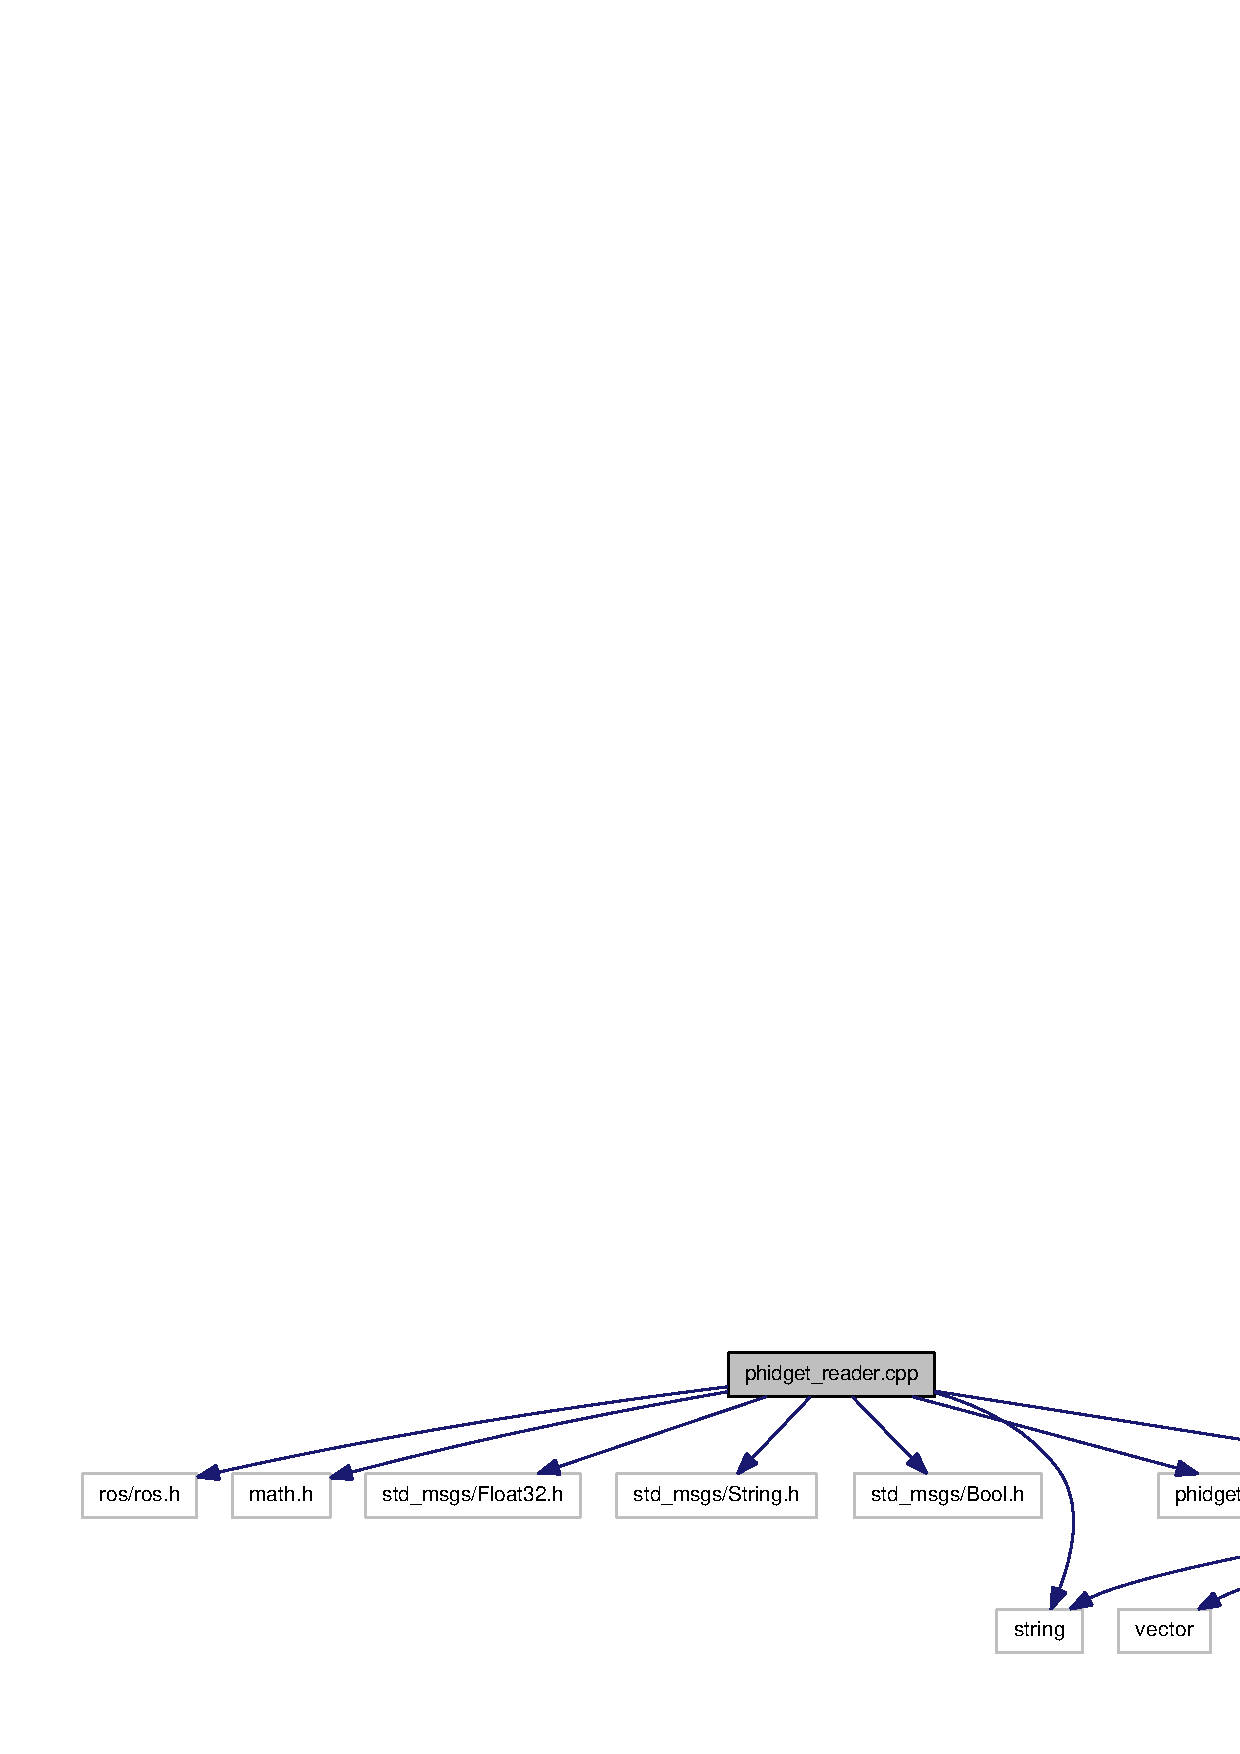
\includegraphics[width=350pt]{phidget__reader_8cpp__incl}
\end{center}
\end{figure}
\subsection*{Functions}
\begin{DoxyCompactItemize}
\item 
int {\bf main} (int argc, char $\ast$$\ast$argv)
\begin{DoxyCompactList}\small\item\em Main method reading the phidget at a specified frequency and smoothing the signal before passing it on. \end{DoxyCompactList}\item 
int {\bf mean} ()
\begin{DoxyCompactList}\small\item\em Method for calulating the mean of the buffer to pass on to the controller. \end{DoxyCompactList}\item 
void {\bf printbuffer} ()
\begin{DoxyCompactList}\small\item\em A small control method to print the buffer. \end{DoxyCompactList}\item 
float {\bf sensor\-To\-Distance} (int sensor\-Value)
\begin{DoxyCompactList}\small\item\em simple calculation method to extract a distance from the sensor value. \end{DoxyCompactList}\item 
void {\bf shift\-Buffer} (int data)
\begin{DoxyCompactList}\small\item\em Method for shifting the buffer and inserting the newest sensor value. \end{DoxyCompactList}\item 
void {\bf shutdown} (const std\-\_\-msgs\-::\-Bool\-::\-Const\-Ptr \&b)
\begin{DoxyCompactList}\small\item\em Controll method to shutdown this R\-O\-S node when the command is given. \end{DoxyCompactList}\end{DoxyCompactItemize}
\subsection*{Variables}
\begin{DoxyCompactItemize}
\item 
int {\bf buffer} [{\bf buffer\-\_\-size}]
\item 
const int {\bf buffer\-\_\-size} = 25
\item 
const int {\bf freq} = 250
\item 
const int {\bf sensor\-\_\-id} = 4
\end{DoxyCompactItemize}


\subsection{Function Documentation}
\index{phidget\-\_\-reader.\-cpp@{phidget\-\_\-reader.\-cpp}!main@{main}}
\index{main@{main}!phidget_reader.cpp@{phidget\-\_\-reader.\-cpp}}
\subsubsection[{main}]{\setlength{\rightskip}{0pt plus 5cm}int main (
\begin{DoxyParamCaption}
\item[{int}]{argc, }
\item[{char $\ast$$\ast$}]{argv}
\end{DoxyParamCaption}
)}\label{phidget__reader_8cpp_a3c04138a5bfe5d72780bb7e82a18e627}


Main method reading the phidget at a specified frequency and smoothing the signal before passing it on. 

Here the phidget is read at a fixed interval, given by freq. These values are stored in the buffer and sliding mean smoothing is applied. This ensures a less spikey signal for the controller and impulses are filtered out. This also means that the system has a longer response time, but by increasing the frequency this is nullified. The buffer acts as a queue, shifting the values every time before calculating a mean value to pass on to the controller. \begin{DoxySeeAlso}{See Also}
\doxyref{shift\-Buffer(int)}{p.}{phidget__reader_8cpp_ab3f7db7de2a2af54619cd7ac3517b924}, \doxyref{mean()}{p.}{phidget__reader_8cpp_a478ef96a3ad4032e1f91152178c8809e} 
\end{DoxySeeAlso}


Definition at line 32 of file phidget\-\_\-reader.\-cpp.

\index{phidget\-\_\-reader.\-cpp@{phidget\-\_\-reader.\-cpp}!mean@{mean}}
\index{mean@{mean}!phidget_reader.cpp@{phidget\-\_\-reader.\-cpp}}
\subsubsection[{mean}]{\setlength{\rightskip}{0pt plus 5cm}int mean (
\begin{DoxyParamCaption}
{}
\end{DoxyParamCaption}
)}\label{phidget__reader_8cpp_a478ef96a3ad4032e1f91152178c8809e}


Method for calulating the mean of the buffer to pass on to the controller. 

This method calculated the mean of the values in the buffer. \begin{DoxyReturn}{Returns}
The calculated mean. 
\end{DoxyReturn}
\begin{DoxySeeAlso}{See Also}
\doxyref{shift\-Buffer(int)}{p.}{phidget__reader_8cpp_ab3f7db7de2a2af54619cd7ac3517b924} 
\end{DoxySeeAlso}


Definition at line 97 of file phidget\-\_\-reader.\-cpp.

\index{phidget\-\_\-reader.\-cpp@{phidget\-\_\-reader.\-cpp}!printbuffer@{printbuffer}}
\index{printbuffer@{printbuffer}!phidget_reader.cpp@{phidget\-\_\-reader.\-cpp}}
\subsubsection[{printbuffer}]{\setlength{\rightskip}{0pt plus 5cm}void printbuffer (
\begin{DoxyParamCaption}
{}
\end{DoxyParamCaption}
)}\label{phidget__reader_8cpp_a09b9cf5195215cdfaa34111afd03c8a8}


A small control method to print the buffer. 

Prints the buffer for each iteration so the calculated mean value can be evaluated. \begin{DoxySeeAlso}{See Also}
\doxyref{mean()}{p.}{phidget__reader_8cpp_a478ef96a3ad4032e1f91152178c8809e} 
\end{DoxySeeAlso}


Definition at line 111 of file phidget\-\_\-reader.\-cpp.

\index{phidget\-\_\-reader.\-cpp@{phidget\-\_\-reader.\-cpp}!sensor\-To\-Distance@{sensor\-To\-Distance}}
\index{sensor\-To\-Distance@{sensor\-To\-Distance}!phidget_reader.cpp@{phidget\-\_\-reader.\-cpp}}
\subsubsection[{sensor\-To\-Distance}]{\setlength{\rightskip}{0pt plus 5cm}float sensor\-To\-Distance (
\begin{DoxyParamCaption}
\item[{int}]{sensor\-Value}
\end{DoxyParamCaption}
)}\label{phidget__reader_8cpp_a8564fe398b4af80bdf3877410ffcbc67}


simple calculation method to extract a distance from the sensor value. 

This method converts the sersorvalue to a distance.


\begin{DoxyParams}{Parameters}
{\em sensor\-Value} & The value of the sensor. \\
\hline
\end{DoxyParams}
\begin{DoxyReturn}{Returns}
The calculated distance. 
\end{DoxyReturn}


Definition at line 127 of file phidget\-\_\-reader.\-cpp.

\index{phidget\-\_\-reader.\-cpp@{phidget\-\_\-reader.\-cpp}!shift\-Buffer@{shift\-Buffer}}
\index{shift\-Buffer@{shift\-Buffer}!phidget_reader.cpp@{phidget\-\_\-reader.\-cpp}}
\subsubsection[{shift\-Buffer}]{\setlength{\rightskip}{0pt plus 5cm}void shift\-Buffer (
\begin{DoxyParamCaption}
\item[{int}]{data}
\end{DoxyParamCaption}
)}\label{phidget__reader_8cpp_ab3f7db7de2a2af54619cd7ac3517b924}


Method for shifting the buffer and inserting the newest sensor value. 

This method shifts all the data elements in the buffer to make place for the new sensor data. The buffer is initialised as an array filled with '1', so the first buffer\-\_\-size values will be invalid. 
\begin{DoxyParams}{Parameters}
{\em data} & The new sensor value to be shifted into the buffer. \\
\hline
\end{DoxyParams}
\begin{DoxySeeAlso}{See Also}
\doxyref{mean()}{p.}{phidget__reader_8cpp_a478ef96a3ad4032e1f91152178c8809e} 
\end{DoxySeeAlso}


Definition at line 84 of file phidget\-\_\-reader.\-cpp.

\index{phidget\-\_\-reader.\-cpp@{phidget\-\_\-reader.\-cpp}!shutdown@{shutdown}}
\index{shutdown@{shutdown}!phidget_reader.cpp@{phidget\-\_\-reader.\-cpp}}
\subsubsection[{shutdown}]{\setlength{\rightskip}{0pt plus 5cm}void shutdown (
\begin{DoxyParamCaption}
\item[{const std\-\_\-msgs\-::\-Bool\-::\-Const\-Ptr \&}]{b}
\end{DoxyParamCaption}
)}\label{phidget__reader_8cpp_a6099bcde46c020c0703be2c28a4432d5}


Controll method to shutdown this R\-O\-S node when the command is given. 

This method will shutdown this node when the command is given by the console. 
\begin{DoxyParams}{Parameters}
{\em b} & The message containing the command. Nothing is done with the command since we know what it will be when this message is received. \\
\hline
\end{DoxyParams}


\subsection{Variable Documentation}
\index{phidget\-\_\-reader.\-cpp@{phidget\-\_\-reader.\-cpp}!buffer@{buffer}}
\index{buffer@{buffer}!phidget_reader.cpp@{phidget\-\_\-reader.\-cpp}}
\subsubsection[{buffer}]{\setlength{\rightskip}{0pt plus 5cm}int buffer[{\bf buffer\-\_\-size}]}\label{phidget__reader_8cpp_a87f0aec3ac049be255616effe0efdc43}
The buffer used for smoothing. 

Definition at line 21 of file phidget\-\_\-reader.\-cpp.

\index{phidget\-\_\-reader.\-cpp@{phidget\-\_\-reader.\-cpp}!buffer\-\_\-size@{buffer\-\_\-size}}
\index{buffer\-\_\-size@{buffer\-\_\-size}!phidget_reader.cpp@{phidget\-\_\-reader.\-cpp}}
\subsubsection[{buffer\-\_\-size}]{\setlength{\rightskip}{0pt plus 5cm}const int buffer\-\_\-size = 25}\label{phidget__reader_8cpp_a9bd822a4ae927624f7827c898422d1db}
Value buffer size for signal smoothing. 

Definition at line 20 of file phidget\-\_\-reader.\-cpp.

\index{phidget\-\_\-reader.\-cpp@{phidget\-\_\-reader.\-cpp}!freq@{freq}}
\index{freq@{freq}!phidget_reader.cpp@{phidget\-\_\-reader.\-cpp}}
\subsubsection[{freq}]{\setlength{\rightskip}{0pt plus 5cm}const int freq = 250}\label{phidget__reader_8cpp_a323a9f2cf2eeae7e0acd9fe48da80fff}
The frequency at which the sensor should be read and the value passed on. 

Definition at line 19 of file phidget\-\_\-reader.\-cpp.

\index{phidget\-\_\-reader.\-cpp@{phidget\-\_\-reader.\-cpp}!sensor\-\_\-id@{sensor\-\_\-id}}
\index{sensor\-\_\-id@{sensor\-\_\-id}!phidget_reader.cpp@{phidget\-\_\-reader.\-cpp}}
\subsubsection[{sensor\-\_\-id}]{\setlength{\rightskip}{0pt plus 5cm}const int sensor\-\_\-id = 4}\label{phidget__reader_8cpp_acdd8c9ca04f3c952e0a17260cfa8f2eb}
The sensor I\-D. 

Definition at line 18 of file phidget\-\_\-reader.\-cpp.


\section{rviz\-\_\-gripper.\-cpp File Reference}
\label{rviz__gripper_8cpp}\index{rviz\-\_\-gripper.\-cpp@{rviz\-\_\-gripper.\-cpp}}
{\ttfamily \#include $<$ros/ros.\-h$>$}\\*
{\ttfamily \#include $<$string$>$}\\*
{\ttfamily \#include $<$std\-\_\-msgs/\-Float32.\-h$>$}\\*
{\ttfamily \#include $<$std\-\_\-msgs/\-Bool.\-h$>$}\\*
{\ttfamily \#include $<$sensor\-\_\-msgs/\-Joint\-State.\-h$>$}\\*
Include dependency graph for rviz\-\_\-gripper.\-cpp\-:\nopagebreak
\begin{figure}[H]
\begin{center}
\leavevmode
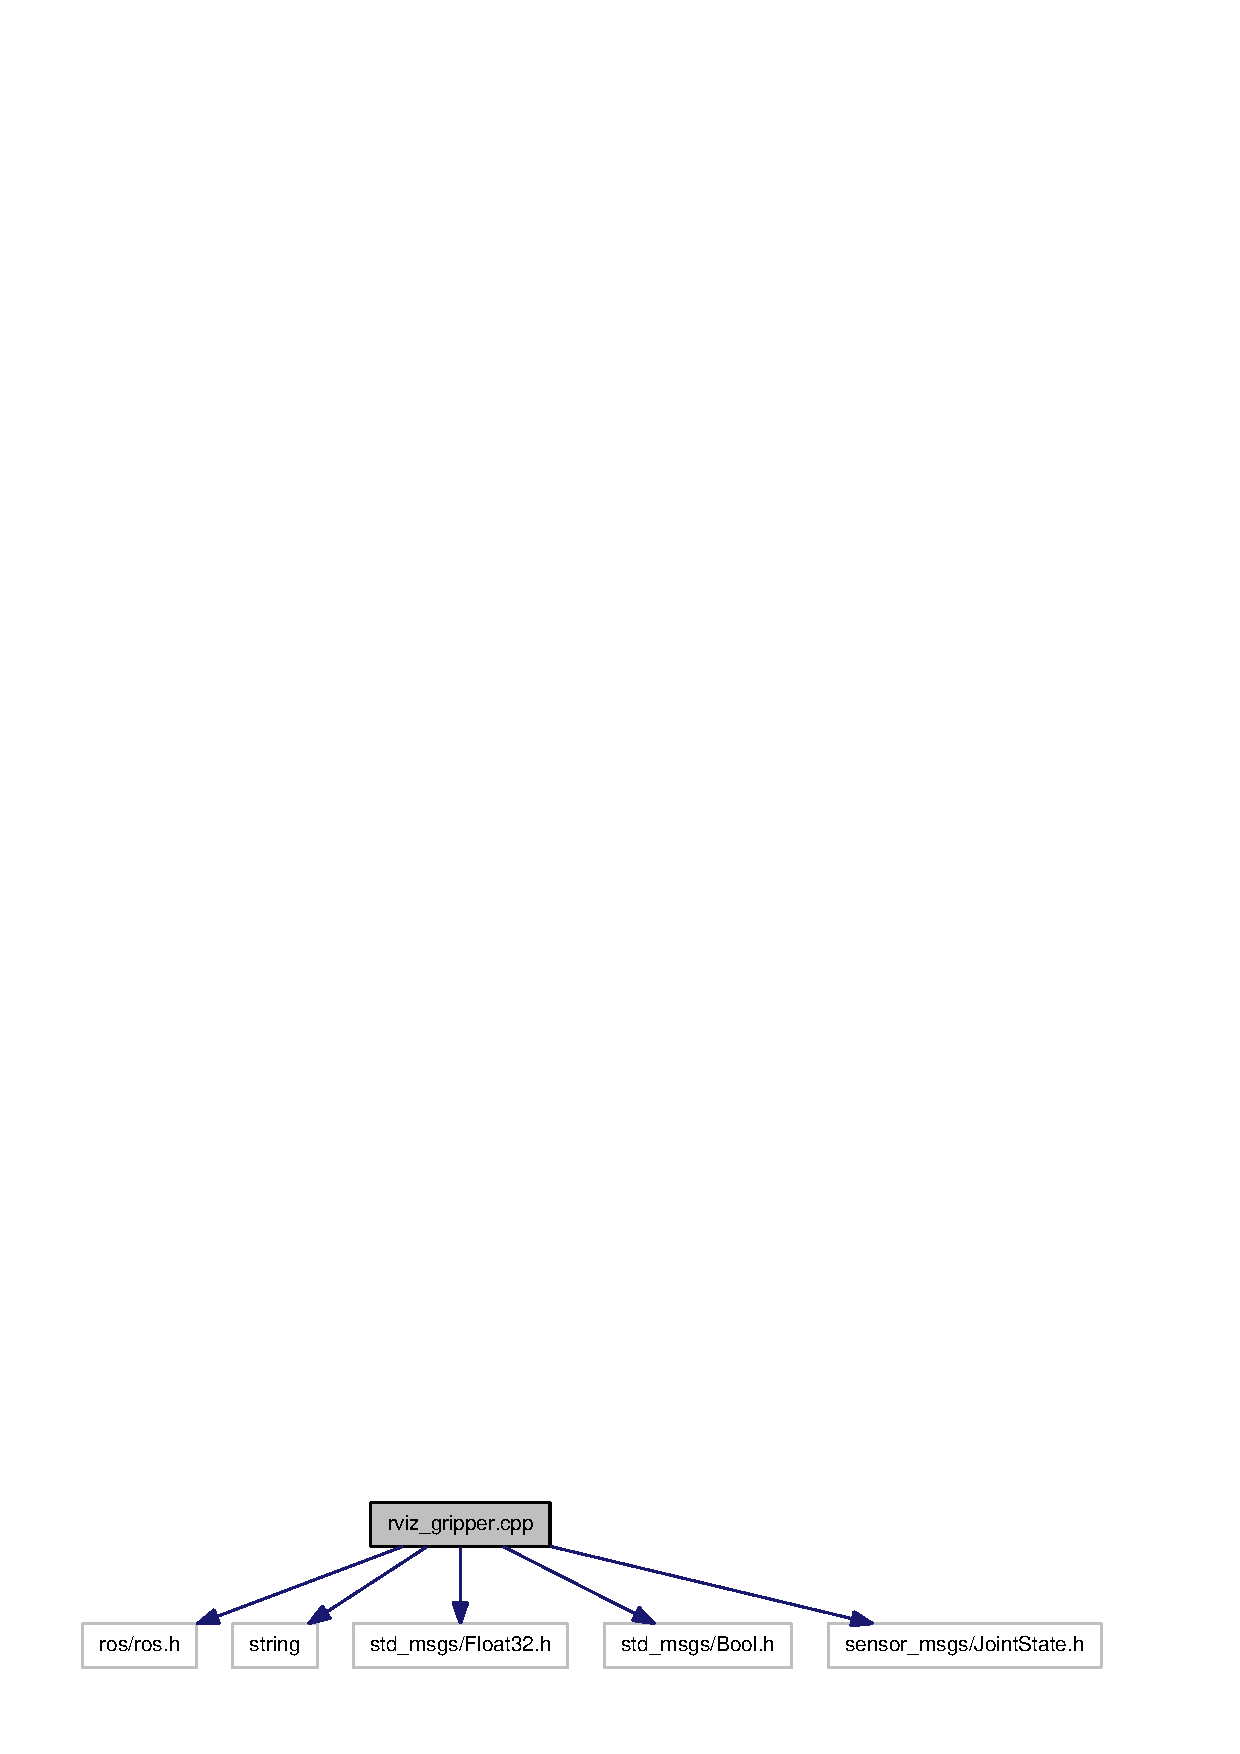
\includegraphics[width=350pt]{rviz__gripper_8cpp__incl}
\end{center}
\end{figure}
\subsection*{Functions}
\begin{DoxyCompactItemize}
\item 
int {\bf main} (int argc, char $\ast$$\ast$argv)
\item 
void {\bf rviz\-Updater} (const std\-\_\-msgs\-::\-Float32\-::\-Const\-Ptr \&)
\item 
void {\bf shutdown} (const std\-\_\-msgs\-::\-Bool\-::\-Const\-Ptr \&)
\end{DoxyCompactItemize}
\subsection*{Variables}
\begin{DoxyCompactItemize}
\item 
float {\bf motor\-\_\-stand}
\end{DoxyCompactItemize}


\subsection{Function Documentation}
\index{rviz\-\_\-gripper.\-cpp@{rviz\-\_\-gripper.\-cpp}!main@{main}}
\index{main@{main}!rviz_gripper.cpp@{rviz\-\_\-gripper.\-cpp}}
\subsubsection[{main}]{\setlength{\rightskip}{0pt plus 5cm}int main (
\begin{DoxyParamCaption}
\item[{int}]{argc, }
\item[{char $\ast$$\ast$}]{argv}
\end{DoxyParamCaption}
)}\label{rviz__gripper_8cpp_a3c04138a5bfe5d72780bb7e82a18e627}


Definition at line 14 of file rviz\-\_\-gripper.\-cpp.

\index{rviz\-\_\-gripper.\-cpp@{rviz\-\_\-gripper.\-cpp}!rviz\-Updater@{rviz\-Updater}}
\index{rviz\-Updater@{rviz\-Updater}!rviz_gripper.cpp@{rviz\-\_\-gripper.\-cpp}}
\subsubsection[{rviz\-Updater}]{\setlength{\rightskip}{0pt plus 5cm}void rviz\-Updater (
\begin{DoxyParamCaption}
\item[{const std\-\_\-msgs\-::\-Float32\-::\-Const\-Ptr \&}]{msg}
\end{DoxyParamCaption}
)}\label{rviz__gripper_8cpp_a82df680c1afd396b56d422518e69df6d}


Definition at line 76 of file rviz\-\_\-gripper.\-cpp.

\index{rviz\-\_\-gripper.\-cpp@{rviz\-\_\-gripper.\-cpp}!shutdown@{shutdown}}
\index{shutdown@{shutdown}!rviz_gripper.cpp@{rviz\-\_\-gripper.\-cpp}}
\subsubsection[{shutdown}]{\setlength{\rightskip}{0pt plus 5cm}void shutdown (
\begin{DoxyParamCaption}
\item[{const std\-\_\-msgs\-::\-Bool\-::\-Const\-Ptr \&}]{b}
\end{DoxyParamCaption}
)}\label{rviz__gripper_8cpp_a9eeee6c84a027eabdd7230329be56bec}


\subsection{Variable Documentation}
\index{rviz\-\_\-gripper.\-cpp@{rviz\-\_\-gripper.\-cpp}!motor\-\_\-stand@{motor\-\_\-stand}}
\index{motor\-\_\-stand@{motor\-\_\-stand}!rviz_gripper.cpp@{rviz\-\_\-gripper.\-cpp}}
\subsubsection[{motor\-\_\-stand}]{\setlength{\rightskip}{0pt plus 5cm}float motor\-\_\-stand}\label{rviz__gripper_8cpp_a4d33c6d3680f82ddfa464ba1739b851a}


Definition at line 12 of file rviz\-\_\-gripper.\-cpp.


\section{rviz\-\_\-object.\-cpp File Reference}
\label{rviz__object_8cpp}\index{rviz\-\_\-object.\-cpp@{rviz\-\_\-object.\-cpp}}
{\ttfamily \#include \char`\"{}ros/ros.\-h\char`\"{}}\\*
{\ttfamily \#include \char`\"{}std\-\_\-msgs/\-Int32.\-h\char`\"{}}\\*
{\ttfamily \#include $<$sstream$>$}\\*
Include dependency graph for rviz\-\_\-object.\-cpp\-:
\nopagebreak
\begin{figure}[H]
\begin{center}
\leavevmode
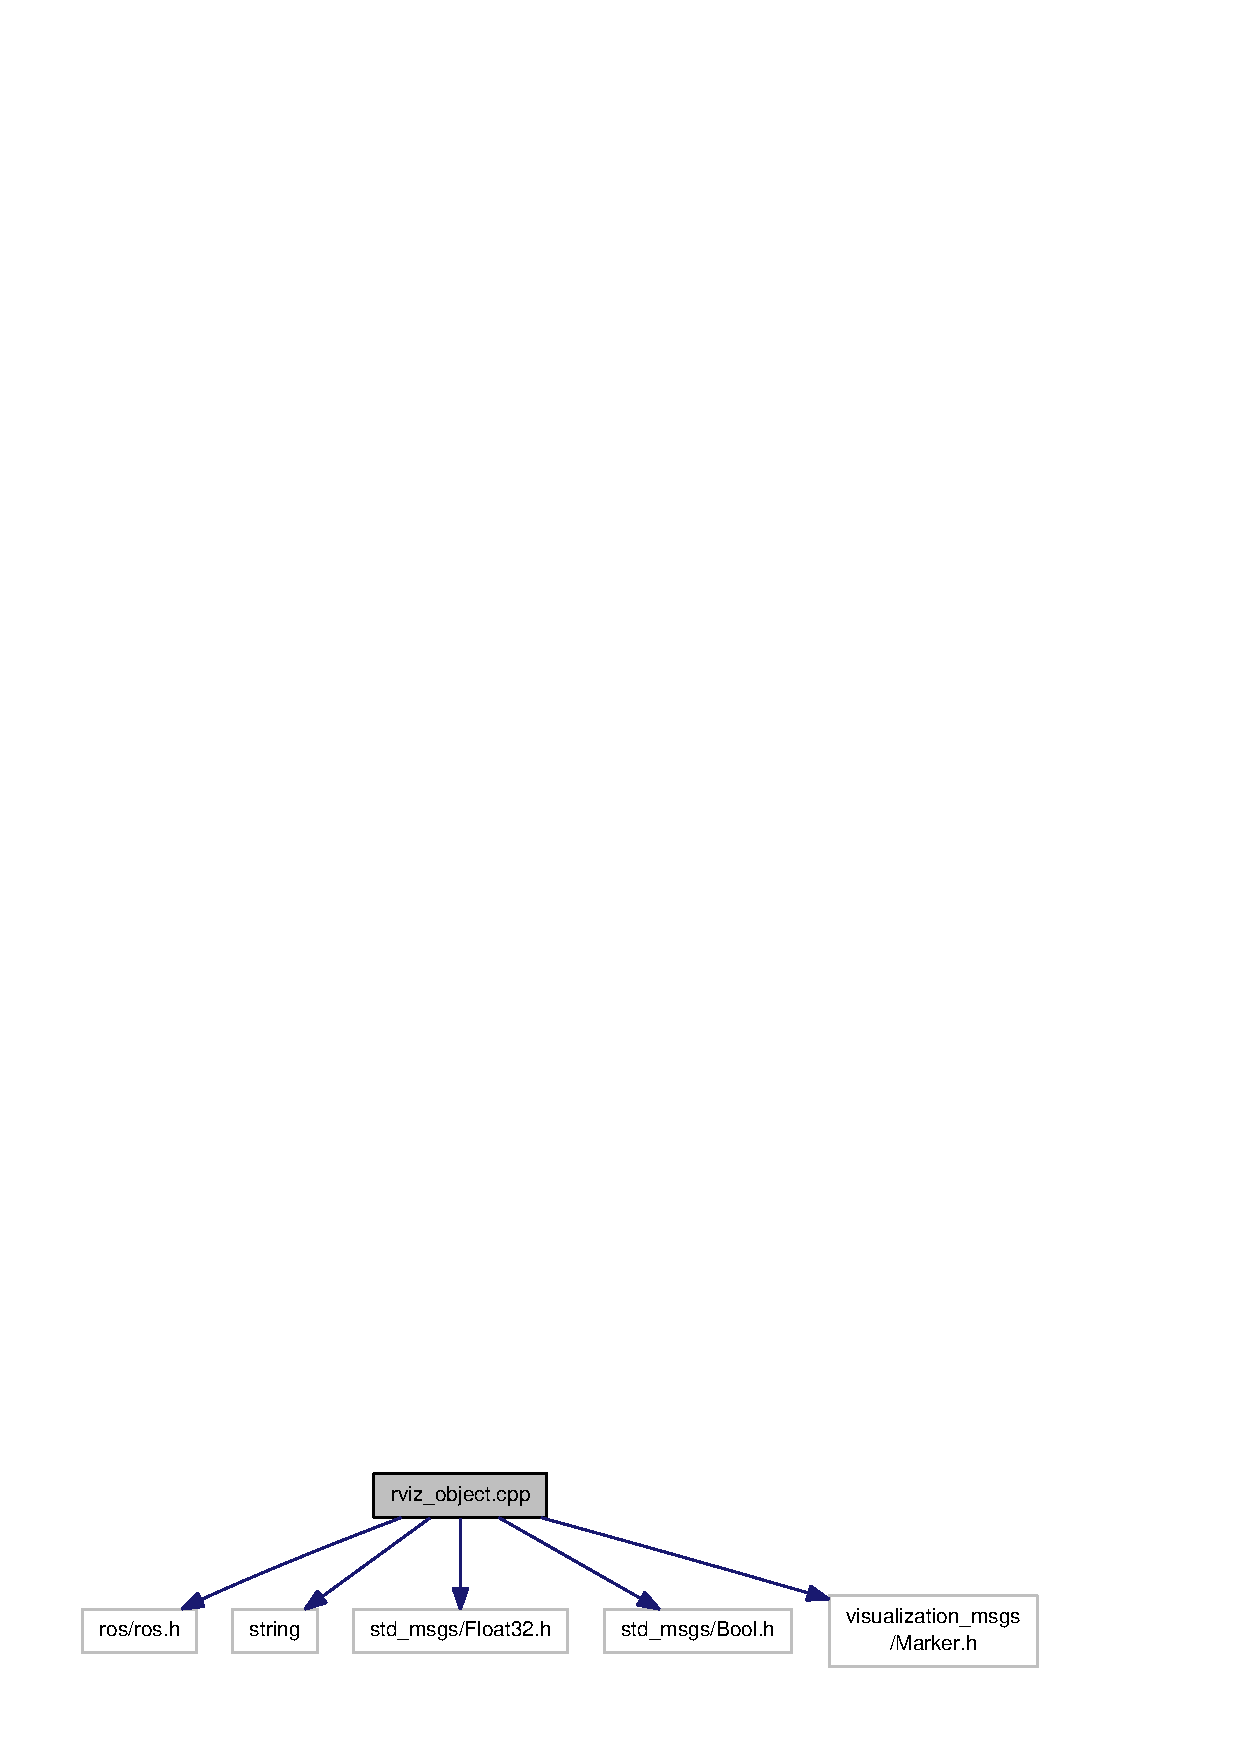
\includegraphics[width=278pt]{rviz__object_8cpp__incl}
\end{center}
\end{figure}
\subsection*{Functions}
\begin{DoxyCompactItemize}
\item 
int {\bf main} (int argc, char $\ast$$\ast$argv)
\item 
void {\bf rviz\-Updater} ()
\item 
void {\bf rviz\-Updater} (const std\-\_\-msgs\-::\-Int32\-::\-Const\-Ptr \&msg)
\end{DoxyCompactItemize}


\subsection{Function Documentation}
\index{rviz\-\_\-object.\-cpp@{rviz\-\_\-object.\-cpp}!main@{main}}
\index{main@{main}!rviz_object.cpp@{rviz\-\_\-object.\-cpp}}
\subsubsection[{main}]{\setlength{\rightskip}{0pt plus 5cm}int main (
\begin{DoxyParamCaption}
\item[{int}]{argc, }
\item[{char $\ast$$\ast$}]{argv}
\end{DoxyParamCaption}
)}\label{rviz__object_8cpp_a3c04138a5bfe5d72780bb7e82a18e627}


Definition at line 7 of file rviz\-\_\-object.\-cpp.

\index{rviz\-\_\-object.\-cpp@{rviz\-\_\-object.\-cpp}!rviz\-Updater@{rviz\-Updater}}
\index{rviz\-Updater@{rviz\-Updater}!rviz_object.cpp@{rviz\-\_\-object.\-cpp}}
\subsubsection[{rviz\-Updater}]{\setlength{\rightskip}{0pt plus 5cm}void rviz\-Updater (
\begin{DoxyParamCaption}
{}
\end{DoxyParamCaption}
)}\label{rviz__object_8cpp_a1ce015110fa95736c5c473f56d8740a4}
\index{rviz\-\_\-object.\-cpp@{rviz\-\_\-object.\-cpp}!rviz\-Updater@{rviz\-Updater}}
\index{rviz\-Updater@{rviz\-Updater}!rviz_object.cpp@{rviz\-\_\-object.\-cpp}}
\subsubsection[{rviz\-Updater}]{\setlength{\rightskip}{0pt plus 5cm}void rviz\-Updater (
\begin{DoxyParamCaption}
\item[{const std\-\_\-msgs\-::\-Int32\-::\-Const\-Ptr \&}]{msg}
\end{DoxyParamCaption}
)}\label{rviz__object_8cpp_a31e2e60662d5ec68828a3372cd4f22b7}


Definition at line 17 of file rviz\-\_\-object.\-cpp.


\addcontentsline{toc}{part}{Index}
\printindex
\end{document}
